\renewcommand{\NomeBloco}{APS\_digitalized}
\renewcommand{\NomeBlocoNoUnderline}{apsdigitalized}
\renewcommand{\NomePTab}{tab_\NomeBlocoNoUnderline}
\renewcommand{\NomeSTab}{tab_\NomeBlocoNoUnderline2}
\renewcommand{\NomePFig}{fig_\NomeBlocoNoUnderline}
\renewcommand{\NomeSFig}{fig_\NomeBlocoNoUnderline2}
\renewcommand{\NomeTTab}{tab_\NomeBlocoNoUnderline3}
\renewcommand{\NomeQTab}{tab_\NomeBlocoNoUnderline4}

\section{\NomeBloco}

O \emph{APS\_digitalized} \'e o circuito respons\'avel por digitalizar o sinal gerado pelo APS descrito na \autoref{section:APS}. O bloco apresenta as defini{\c c}\~oes de sinais de entrada e sa\'ida referidos na \autoref{\NomeSTab}.

\begin{table}[htbp]
\caption{Sinais do bloco \NomeBloco}
\label{\NomeSTab}
\centering
\begin{tabular}{ccll}

    \toprule
    Sinal & Tipo    & Descri{\c c}\~ao & Observa{\c c}\~ao        \\
    \midrule \midrule
    RESET   & Entrada   & Sinal de RESET no APS & Ativo em nível baixo\\
    \midrule
    ENABLE   & Entrada   & Sinal de ENABLE no APS & Ativo em nível alto\\
    \midrule
    Vref   & Entrada   & Tens\~ao de refer\^encia utilizada pelo comparador \\
    \midrule
    Ibias   & Entrada   & Corrente de polariza{\c c}\~ao do comparador \\
    \midrule
    AnOut   & Saída   & Sinal anal\'ogico produzido pelo APS \\
    \midrule
    DigOut   & Saída   & Sinal digital produzido pelo Comparador \\
    \bottomrule
\end{tabular}
\legend{Fonte: Produzido pelo autor}
\end{table}

O circuito projetado para o bloco \'e demonstrado na \autoref{\NomePFig}.

\begin{figure}[htb]
 \label{\NomePFig}
 \centering
    \centering
    \caption{Circuito CMOS projetado para o bloco \NomeBloco} 
    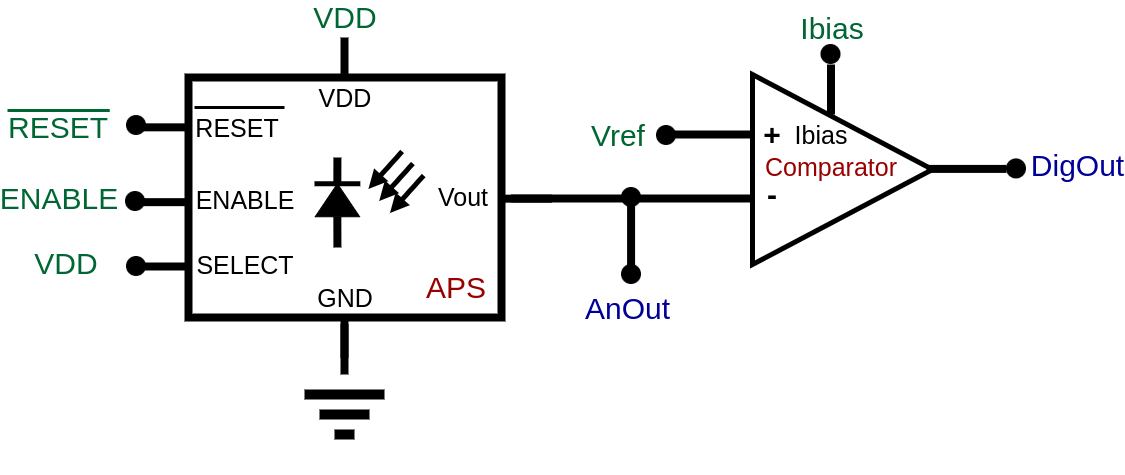
\includegraphics[scale=0.4]{Circuitos/APS_digitalized.png}
    \legend{Fonte: Produzido pelo autor}
\end{figure}

\begin{figure}[htb]
 \centering
    \centering
    \caption{Representa{\c c}\~ao em bloco do \NomeBloco} \label{\NomeSFig}
    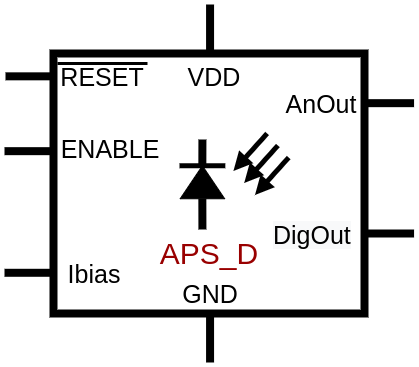
\includegraphics[scale=0.5]{Circuitos/APS_digitalized_block.png}
    \legend{Fonte: Produzido pelo autor}
\end{figure}

A sa\'ida digital do bloco funciona realizando uma compara{c c}\~ao entre uma tens\~ao de refer\^encia chamada de \emph{Vref} e a sa\'ida anal\'ogica do APS, chamada de \emph{AnOut}. Quando o valor de \emph{Vref} for maior do que o de \emph{AnOut}, o comparador ir\'a saturar e apresentar em a m\'axima tens\~ao na sa\'ida, que deve ser aproximamente igual a \emph{VDD}, interpretada como n\'ivel l\'ogico '1'. Quando o valor de \emph{Vref} for menor ou igual do que o de \emph{AnOut}, o comparador ir\'a apresentar um sinal de aproximadamente \emph{GND} em sua sa\'ida, interpretada como n\'ivel l\'ogico '0'.
Utilizando o elemento comparador, podemos ajustar para que a sa\'ida retorne '0' apenas quando for atingido um valor limiar controlado. Como sabemos que a intensidade da corrente fotogerada depende da intensidade da luz captada pelo fotodiodo (\autoref{secao_fotodiodo}), podemos deduzir a informa{\c c}\~ao sobre intensidade luminosa verificando em quanto tempo demora para que se mude de n\'ivel l\'ogico '1' para '0' durante o Est\'agio 2, utilizando-se a \autoref{eq_responsividade} e a \autoref{eq_modEletFotIl} e para se obter a \autoref{eq_apsd}.

\begin{equation}
    \label{eq_apsd}
    P = \frac{(VDD-V_{ref})(C_{j}+C_{cn})}{R_{\lambda}T}
\end{equation}

Onde:

\begin{itemize}

    \item \emph{P$_{FD}$} \'e a pot\^encia \'optica presente no fotodiodo [W]
    \item \emph{R$_\lambda$} \'e a Responsividade [A.W$^{-1}$]
    \item \emph{VDD} \'e a tens\~ao de alimenta{\c c}\~ao do circuito [$V$]
    \item \emph{$V_{ref}$} \'e a tens\~ao de refer\^encia do comparador [$V$]
    \item \emph{$C_j$} \'e a capacit\^ancia de jun{\c c}\~ao do fotodiodo [F]
    \item \emph{$C_{cn}$} \'e a capacit\^ancia do n\'o central do APS [F]
    \item $R_{\lambda}$ \'e a responsividade para o comprimento de onda detectado no fotodiodo [$A.W^{-1}$]
    \item \emph{T} \'e o per\'iodo do qual o n\'ivel l\'ogico mudou de '1' para '0' [\emph{s}]
    
\end{itemize}

Um transistor NMOS n\~ao apresentado na ilustra{\c c}\~ao foi conectado com o dreno e fonte ligados ao terra e o gate em VDD, de forma a se formar um capacitor de desacoplamento para o bloco. Os par\^ametros desse transistor s\~ao dadas na \autoref{tab_capdecapsd}.

\begin{table}[htbp]
\caption{Capacitor de desacoplamento via transistor do bloco \NomeBloco}
\label{tab_capdecapsd}
\centering
\begin{tabular}{cccc}
\toprule
W ($\mu$m)  & L ($\mu$m) & M (n° dispositivos) & S (n° dispositivos)\\
\midrule \midrule
10 & 19.995 & 1 & 1\\
\bottomrule
\end{tabular}
\legend{Fonte: Produzido pelo autor}
\end{table}
\clearpage

